\iffalse
\title{Assignment}
\author{ee24btech11064}
\section{integer}
\fi

%\begin{enumerate}
\item $\lim_{x\to2}$ $\frac{3^x+\frac{27}{3^x}-12}{\frac{1}{3^\frac{x}{2}}-\frac{3}{3^x}}$ is equal to.
\hfill[Jan 2020]
\item If variance of first $n$ natural numbers is $10$ and variance of first $m$ even natural numbers is $16$, $m + n$ is equal to
\hfill[Jan 2020]
\item  If the sum of the coefficients of all even powers of $x$ in the product
\begin{align*}
    \brak{1+x+x^2+x^3\cdots+x^{2n}}\brak{1-x+x^2-x^3\cdots+x^{2n}}
\end{align*}
is $61$, then $n$ is equal to \hfill[Jan 2020]
\item Let $S$ be the set of points where the function, $f\brak{x}=|2-|x-3||$, $x \in R$, is not differentiable. Then, the value of $\sum x \in S f\brak{f\brak{x}}$ is equal to
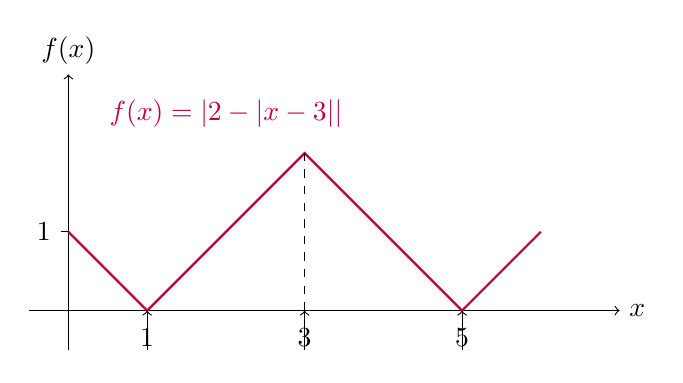
\begin{tikzpicture}

% Draw axes
\draw[->] (-0.5,0) -- (7,0) node[right] {$x$};
\draw[->] (0,-0.5) -- (0,3) node[above] {$f(x)$};

% Plot the function
\draw[thick, purple, domain=0:6] plot(\x, {abs(2 - abs(\x - 3))});

% Label the function
\node[purple] at (2,2.5) {$f(x) = |2 - |x-3||$};

% Add the values on the x-axis
\draw[dashed] (3,0) -- (3,2) node[above right] {};
\foreach \x in {1,3,5} \draw (\x,0) -- (\x,-0.1) node[below] {\x};

% Add the value on the y-axis
\draw (0,1) -- (-0.1,1) node[left] {1};

% Arrows on the x-axis
\foreach \x in {1,3,5}
    \draw[->] (\x, -0.5) -- (\x, 0);

\end{tikzpicture} \hfill[Jan 2020]
\item Let $A\brak{1,0}$, $B\brak{6,2}$, $C\brak{\frac{3}{2},6}$ be the vertices of a triangle $ABC$. If $P$ is a point inside the triangle $ABC$ such that the triangle $APC,APB$ and $BPC$ have equal areas, then the length of the line segment $PQ$, where $Q$ is the point $\brak{\frac{-7}{6},\frac{-1}{3}}$, is \hfill[Jan 2020] 
%\end{enumerate}
